% ================================================================
% figs-batch1.tex —— 讲义手绘示意图的 TikZ 重绘（第 1 批，共 9 幅）
% 覆盖 p.10, p.11（2 幅）, p.24, p.43（2 幅）, p.44, p.45, p.50。
% 只含图体（tikzpicture），不含 figure 环境与 caption，不引用外部图片。
%
% 命名：\figP<页>-<序>。LaTeX 控制序列名不能含数字，直接写 \newcommand{\figP010}
% 会报错（控制序列被截断），故一律用 \csname 定义；正文调用写
%   \figP{010}、\figP{011-1}、\figP{043-2} …（文件末尾的 \figP 转发），
% 或直接写 \csname figP010\endcsname。
% ================================================================

% p.10：闭环单位圆盘 $\mathbb B_C$ 内的环带 $\mathbb A(\epsilon,r)$（灰色阴影），圆心穿孔标 ×
\expandafter\newcommand\csname figP010\endcsname{%
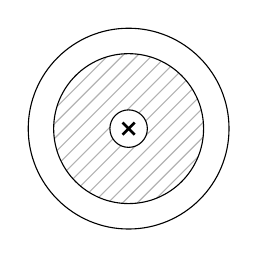
\begin{tikzpicture}[scale=0.85]
  \begin{scope}
    \clip (0,0) circle (1.12);
    \foreach \y in {-1.9,-1.68,...,1.9}
      \draw[gray!60] (-1.6,\y-1.6) -- (1.6,\y+1.6);
  \end{scope}
  \fill[white] (0,0) circle (0.28);
  \draw (0,0) circle (1.5);
  \draw (0,0) circle (1.12);
  \draw (0,0) circle (0.28);
  \draw[line width=0.9pt] (-0.09,-0.09)--(0.09,0.09) (0.09,-0.09)--(-0.09,0.09);
\end{tikzpicture}}

% p.11：Frobenius $\phi_C$ 在 $\mathbb D_C^\times$ 上的自由、真不连续作用：每点沿轨道向外移动
\expandafter\newcommand\csname figP011-1\endcsname{%
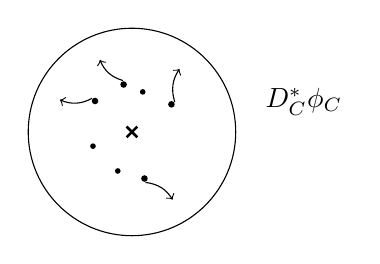
\begin{tikzpicture}[scale=0.85]
  \draw (0,0) circle (1.55);
  \draw[line width=0.9pt] (-0.08,-0.08)--(0.08,0.08) (0.08,-0.08)--(-0.08,0.08);
  \foreach \a/\da in {140/16, 100/14, 35/18, 285/16} {
    \fill (\a:0.72) circle (1.4pt);
    \draw[->] (\a:0.78) to[bend left=25] (\a+\da:1.18);
  }
  \foreach \a in {75, 200, 250} \fill (\a:0.62) circle (1.2pt);
  \node[right] at (1.85,0.45) {$\mathbb D_C^*\curvearrowright\phi_C$};
\end{tikzpicture}}

% p.11：环带 $\mathbb A(r,r^{1/q})$ 上 Frobenius 把内边界点送往外边界点；下方为商 $X_{C,E}$（环面）
\expandafter\newcommand\csname figP011-2\endcsname{%
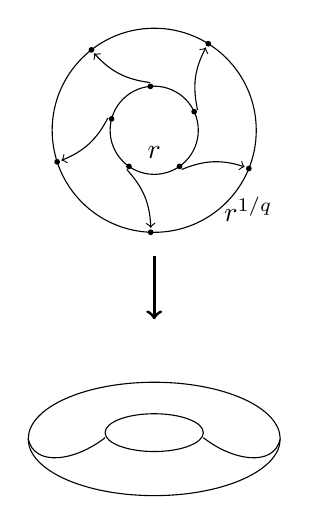
\begin{tikzpicture}[scale=0.8]
  \draw (0,0) circle (1.62);
  \draw (0,0) circle (0.7);
  \foreach \a in {25, 95, 165, 235, 305} {
    \fill (\a:0.7) circle (1.3pt);
    \fill (\a+33:1.62) circle (1.3pt);
    \draw[->] (\a:0.76) to[bend left=20] (\a+33:1.55);
  }
  \node at (270:0.35) {$r$};
  \node at (320:1.95) {$r^{1/q}$};
  \draw[->, line width=1.1pt] (0,-2.0) -- (0,-3.0);
  \begin{scope}[shift={(0,-4.9)}]
    \draw (0,0) ellipse (2.0 and 0.9);
    \draw (0,0.10) ellipse (0.78 and 0.30);
    \draw (-2.0,0) .. controls (-1.9,-0.45) and (-1.25,-0.35) .. (-0.78,0.02);
    \draw (2.0,0) .. controls (1.9,-0.45) and (1.25,-0.35) .. (0.78,0.02);
  \end{scope}
\end{tikzpicture}}

% p.24：Warning 5.6 的图——分歧映射的曲线（源曲线蛇形覆于底曲线之上，分歧点处打孔）
\expandafter\newcommand\csname figP024\endcsname{%
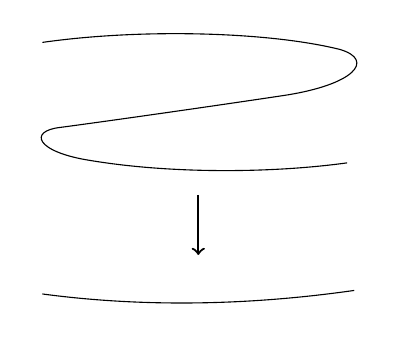
\begin{tikzpicture}[scale=0.9]
  \draw (-2.2,2.45) .. controls (-0.8,2.65) and (1.0,2.6) .. (2.0,2.35)
        .. controls (2.5,2.2) and (2.2,1.85) .. (1.2,1.7)
        .. controls (0.2,1.55) and (-1.2,1.35) .. (-1.95,1.25)
        .. controls (-2.4,1.2) and (-2.3,0.9) .. (-1.5,0.78)
        .. controls (-0.4,0.6) and (1.0,0.6) .. (2.1,0.75);
  \draw[->, line width=0.8pt] (0,0.3) -- (0,-0.55);
  \draw (-2.2,-1.1) .. controls (-0.7,-1.3) and (0.8,-1.25) .. (2.2,-1.05);
\end{tikzpicture}}

% p.43：$\mathcal M_{\mathrm{ell},\mathbf C_p,\infty}$ 经 Hodge–Tate 周期映射到 $\mathbf P^1_{\mathbb Q_p}$；
%        左侧叠层曲线上的两列红盘是超奇异约化的圆盘，下方椭圆上的红盘同此
\expandafter\newcommand\csname figP043-1\endcsname{%
\begin{tikzpicture}[scale=0.8]
  \draw (-3.4,3.45) .. controls (-1.9,3.6) and (-0.2,3.55) .. (0.5,3.35);
  \draw (-3.4,3.0) .. controls (-1.8,3.2) and (-0.1,3.1) .. (0.55,2.95)
        .. controls (0.95,2.85) and (0.8,2.65) .. (0.15,2.65);
  \draw (-3.4,2.55) .. controls (-1.8,2.75) and (0.0,2.6) .. (0.55,2.5)
        .. controls (0.95,2.4) and (0.8,2.2) .. (0.15,2.2);
  \draw (-3.4,2.1) .. controls (-1.7,2.3) and (0.1,2.2) .. (0.6,2.05);
  \draw (-3.4,1.65) .. controls (-1.9,1.8) and (-0.4,1.75) .. (0.4,1.65);
  \foreach \x in {-2.2,-0.9}
    \foreach \y in {3.6,3.26,2.92,2.58,2.24,1.9,1.56,1.22} {
      \fill[red!75] (\x,\y) ellipse (0.27 and 0.16);
      \draw[red!55!black] (\x,\y) ellipse (0.27 and 0.16);
    }
  \draw[->] (0.7,3.45) -- (1.5,3.65);
  \node[right] at (1.55,3.65) {$\mathbf P^1_{\mathbb Q_p}$};
  \node at (3.0,2.4) {$\mathcal M_{\mathrm{ell},\mathbf C_p,\infty}$};
  \draw[->] (3.0,2.0) -- (3.0,1.45);
  \node at (3.0,1.15) {$\mathcal M_{\mathrm{ell},\mathbf C_p}$};
  \draw (-1.6,-0.8) ellipse (1.9 and 0.66);
  \foreach \x/\y in {-2.45/0.2,-1.55/0.42,-0.6/0.15} {
    \draw[red!60!black] (\x,-0.14) -- (\x,\y-0.15);
    \fill[red!75] (\x,\y) ellipse (0.25 and 0.16);
    \draw[red!55!black] (\x,\y) ellipse (0.25 and 0.16);
  }
  \node[red!70!black] at (-1.6,-2.05) {\small 超奇异约化的圆盘};
\end{tikzpicture}}

% p.43：超奇异圆盘的原像（左上不规则区域）经 Hodge–Tate 映射落入
%        $\mathbf P^1_{\mathbf C_p}\setminus\mathbf P^1(\mathbf Q_p)=\Omega^2$；左下椭圆为约化圆盘
\expandafter\newcommand\csname figP043-2\endcsname{%
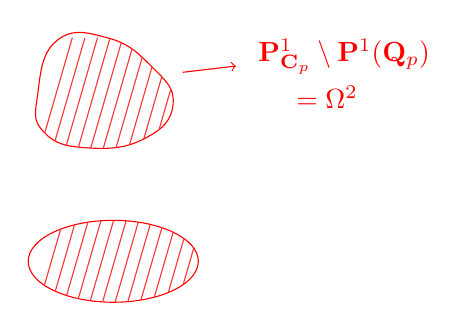
\begin{tikzpicture}[scale=0.8, color=red]
  \draw plot[smooth cycle, tension=0.8] coordinates
    {(-3.3,1.4) (-3.0,2.25) (-2.2,2.3) (-1.5,1.85) (-1.15,1.25) (-1.6,0.7) (-2.5,0.55) (-3.2,0.8)};
  \begin{scope}
    \clip plot[smooth cycle, tension=0.8] coordinates
      {(-3.3,1.4) (-3.0,2.25) (-2.2,2.3) (-1.5,1.85) (-1.15,1.25) (-1.6,0.7) (-2.5,0.55) (-3.2,0.8)};
    \foreach \x in {-3.3,-3.1,...,-1.3} \draw[red!80] (\x,0.4) -- ++(0.55,1.9);
  \end{scope}
  \draw[->] (-1.0,1.75) -- (-0.15,1.85);
  \node[right] at (0.05,2.0) {$\mathbf P^1_{\mathbf C_p}\setminus\mathbf P^1(\mathbf Q_p)$};
  \node[right] at (0.65,1.35) {$=\Omega^2$};
  \draw (-2.1,-1.25) ellipse (1.35 and 0.65);
  \begin{scope}
    \clip (-2.1,-1.25) ellipse (1.35 and 0.65);
    \foreach \x in {-3.3,-3.1,...,-0.9} \draw[red!80] (\x,-2.0) -- ++(0.55,1.9);
  \end{scope}
\end{tikzpicture}}

% p.44：向量丛 $\mathcal E$ 的 Newton 多边形；横轴为 length（秩方向），各级斜率 $\lambda$
%        的重数 $n_\lambda(\xi)$ 决定折点，终点坐标为 $(\mathrm{rank},\mathrm{degree})$
\expandafter\newcommand\csname figP044\endcsname{%
\begin{tikzpicture}[scale=0.85]
  \draw (-1.2,0) -- (6.2,0);
  \draw (0,-1.9) -- (0,4.0);
  \draw[red, line width=1.1pt] (0,0) -- (2.6,-1.35) -- (4.6,-0.95) -- (5.7,2.85);
  \node[right] at (5.75,2.85) {\small $(\text{秩},\text{次数})$};
  \node at (-0.55,-2.1) {\small 长度};
  \node[right] at (1.0,-2.05) {\small $(\lambda\mapsto n_\lambda(\xi))$};
  \draw[->] (-0.2,-1.8) .. controls (0.05,-1.55) and (0.3,-1.3) .. (0.5,-1.02);
\end{tikzpicture}}

% p.45：例 9.3 的两条 Newton 多边形——$\mathcal O(-\frac12)$（斜率 $-1/2$，端点为 $(2,-1)$）
%        与 $\mathcal O\oplus\mathcal O(-1)$（折点 $(1,-1)$、$(2,-1)$）
\expandafter\newcommand\csname figP045\endcsname{%
\begin{tikzpicture}[scale=0.8]
  \draw (-1.3,4.9) -- (4.2,4.9);
  \draw (0,3.5) -- (0,7.1);
  \draw[red, line width=1.1pt] (0,4.9) -- (2.0,3.9);
  \fill (2.0,3.9) circle (1.3pt);
  \node[above left] at (0,6.95) {$\mathcal O(-\tfrac12)$};
  \node[below left] at (0,4.85) {\scriptsize $(0,0)$};
  \node[below right] at (2.0,3.85) {\scriptsize $(2,-1)$};
  \draw (-1.3,0.2) -- (4.2,0.2);
  \draw (0,-1.3) -- (0,2.3);
  \draw[red, line width=1.1pt] (0,0.2) -- (1.3,-1.1) -- (3.0,-1.1);
  \fill (1.3,-1.1) circle (1.3pt);
  \fill (3.0,-1.1) circle (1.3pt);
  \node[above left] at (0,2.15) {$\mathcal O\oplus\mathcal O(-1)$};
  \node[below left] at (0,0.15) {\scriptsize $(0,0)$};
  \node[below] at (1.3,-1.15) {\scriptsize $(1,-1)$};
  \node[below] at (3.0,-1.15) {\scriptsize $(2,-1)$};
\end{tikzpicture}}

% p.50：宽度为 $n$ 的 Newton 多边形——折点坐标为整数（break points integral），终点为 $(n,d)$
\expandafter\newcommand\csname figP050\endcsname{%
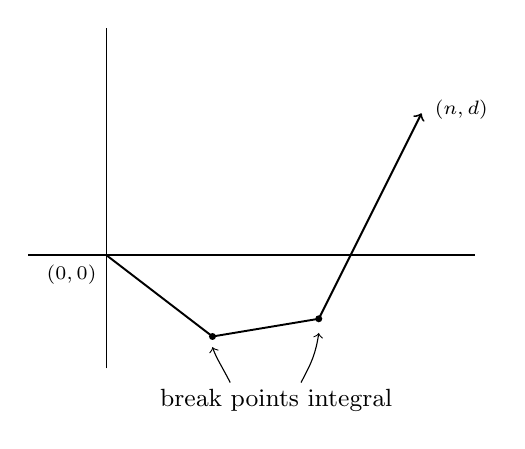
\begin{tikzpicture}[scale=0.9]
  \draw (-1.1,0) -- (5.2,0);
  \draw (0,-1.6) -- (0,3.2);
  \draw[->, line width=0.7pt] (0,0) -- (1.5,-1.15) -- (3.0,-0.9) -- (4.45,2.0);
  \fill (1.5,-1.15) circle (1.4pt);
  \fill (3.0,-0.9) circle (1.4pt);
  \node[below left] at (0,0) {\scriptsize $(0,0)$};
  \node[right] at (4.5,2.05) {\scriptsize $(n,d)$};
  \node at (2.4,-2.05) {\small break points integral};
  \draw[->] (1.75,-1.8) .. controls (1.65,-1.6) and (1.55,-1.45) .. (1.5,-1.3);
  \draw[->] (2.75,-1.8) .. controls (2.85,-1.6) and (2.95,-1.45) .. (3.0,-1.1);
\end{tikzpicture}}

% 转发宏：正文写 \figP{010}、\figP{011-1} 等（用 \providecommand，避免多批文件重复定义）
\providecommand{\figP}[1]{\csname figP#1\endcsname}
